\chapter[Product]{Design and Implementation}
\label{design}

	\section{Introduction}

		Due to the room for research available in this area, it made sense to focus this study on a relatively broad area of the subject to be used as a foundation, rather than to specialise on a particular niche.
		% REWORD THIS?
		Because of this, the main focus for this study is the effects that Non-Euclidean geometry has on a user's sense of Immersion, and to find any changes in a user's comfort navigating in a virtual environment.

		This chapter covers the development process that was undertaken for the creation of the product used for the experiments.

	\section{Development Process}
		% THIS section will cover the development process of the product itself

		% Talk about development methodologies considered for use with the project, and how they were adapted for use for a single person.
			% Use of Git and stuff like that

		% Talk about how you decide to use an existing engine you knew well (save time reinventing the wheel for things like lighting, camera stuff, etc)
		% Also you wanted to limit the amount of outside variables as possible, so an existing engine helped with that

		% Talk about implementation process
			% Started off using render textures, but that had problems regarding depth perception, outside of VR it was fine but inside it was obviously a plane
			% Changed to using render culling and directly viewing the cameras with a bit more tranlation and rotation magics
			% Challenge with multiple variations in how the areas can be set up - angles, inversions on both sides, whether one or both should render, whether you should be able to use it to transport, etc


	\section{Product model}
		% THIS section will contain models of the various states and relations between the functions and other workings of the product, for areas such as the transition between non-Euclidean world areas.
		\autoref{appendix:code:player}

	\begin{figure}[h]
		\label{design:fig:maths}
		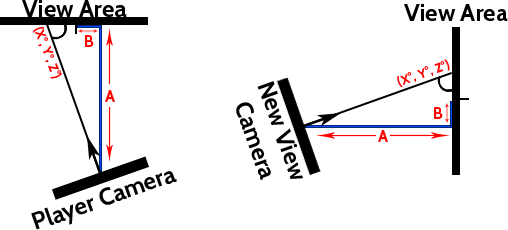
\includegraphics[width=0.8\textwidth]{Images/Position}
		\centering
		\caption{2D representation of the calculations for the position and rotation of cameras.
			See \autoref{appendix:code:camera} for the implementation}
	\end{figure}

	\begin{figure}[h]
		\label{design:fig:scene}
		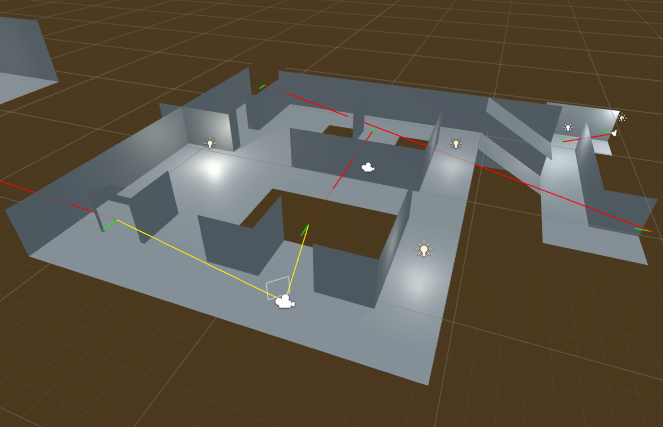
\includegraphics[width=1\textwidth]{Images/Lines_Everywhere2}
		\centering
		\caption{Example view of a scene.
			Red lines are connections between points,
			yellow lines are connections visible to the player,
			and green lines are the direction the connectors are facing}
	\end{figure}

	\begin{figure}[h]
		\label{design:fig:game}
		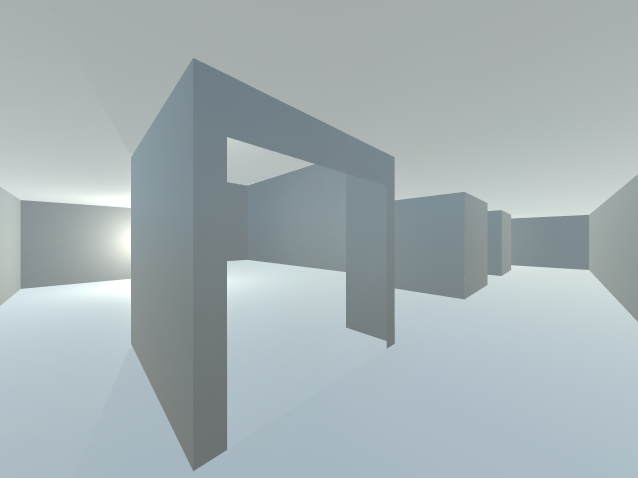
\includegraphics[width=1\textwidth]{Images/NE_View}
		\centering
		\caption{Example of view from inside the Non-Euclidean scene, displaying an area which is larger on the inside}
	\end{figure}

	\section[Environment Design]{Design of experiment environments}
		% HERE I will be covering the designs of the various areas of the virtual environments to be used in the experiments themselves, and why they are applicable for use for the tests.

		% Designed non-Euclidean scene first, ensuring a good mixture of the various types of 'illusions' are displayed effectively
			% Upper right in fig {design:fig:design:ne} is an infinitely repeating corridor, only way out is back where you came from
			% Bottom right connects back to top middle
			% Centre middle creates a shortcut style thing which appers to go through the same space as another corridor
			% Bottom middle appears as if a disproportionally big room is inside a small box
		% Standard Euclidean scene was then created from that scene to create a Euclidean space equivelant, in order to get as close of a comparison between the two as possible to have more consistent results


\begin{figure}[h]
	\label{design:fig:design:ne}
	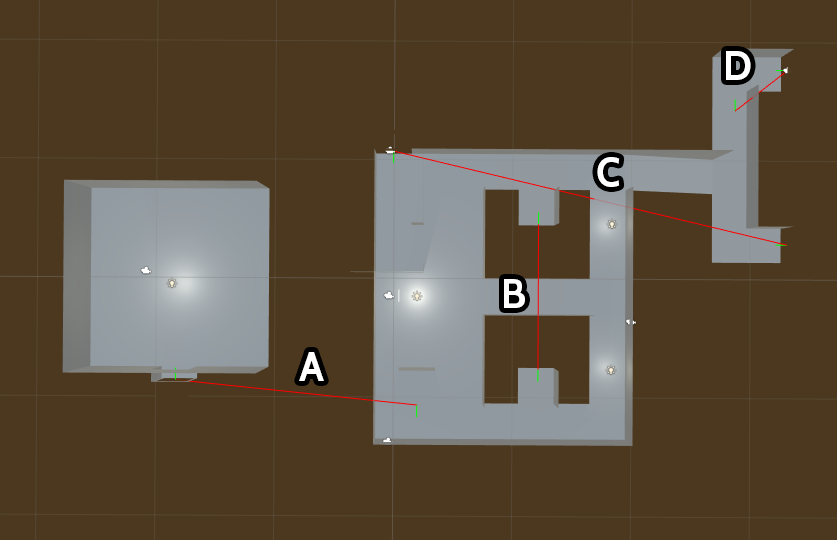
\includegraphics[width=1\textwidth]{Images/NE_Layout}
	\centering
	\caption{Layout of the Non-Euclidean experiment scene}
\end{figure}

\begin{figure}[h]
	\label{design:fig:design:standard}
	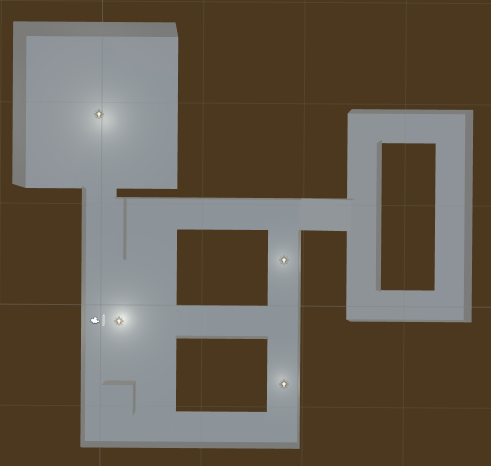
\includegraphics[width=0.7\textwidth]{Images/Standard_Layout}
	\centering
	\caption{Layout of the standard Euclidean experiment scene}
\end{figure}
